% GMGFP
\documentclass{beamer}
\usepackage{caption}
\captionsetup[table]{name=, labelformat = empty, labelsep=newline}

%\usepackage{beamerthemeblackboard}
\usepackage{natbib}
\usepackage{calc}
\usepackage{empheq}
\usepackage{subfig}
\usepackage{siunitx}
\usepackage{fontenc}
\usepackage{amsmath}
\usepackage{array}
\usepackage{wasysym}
\newcolumntype{C}[1]{>{\centering\let\newline\\\arraybackslash\hspace{0pt}}m{#1}}
\newcolumntype{L}[1]{>{\raggedright\let\newline\\\arraybackslash\hspace{0pt}}m{#1}}
\newcolumntype{R}[1]{>{\raggedleft\let\newline\\\arraybackslash\hspace{0pt}}m{#1}}
\usepackage{multirow}
\usepackage[absolute,overlay]{textpos}
%% \usepackage{bbding}
\definecolor{links}{HTML}{2A1B81}
\hypersetup{colorlinks,linkcolor=,urlcolor=links}
\usepackage{listings}
\lstloadlanguages{Matlab}
\lstloadlanguages{C++}
\definecolor{MyDarkGreen}{rgb}{0.0,0.4,0.0}
\lstset{language=C++,
%frame=single,
basicstyle=\small,
tabsize=4,
showstringspaces=false,
numbers=none,
numberstyle=\tiny,
breaklines=true,
firstnumber=1,
language=C++,
basicstyle=\ttfamily,
keywordstyle=\color{blue}\ttfamily,
stringstyle=\color{red}\ttfamily,
commentstyle=\color{gray}\ttfamily,
morecomment=[l][\color{blue}]{\#}
}
\usepackage{tikz}
\usetikzlibrary{arrows,automata}
\usetikzlibrary{positioning}

\newcommand{\ped}[1]{_{\mathrm{#1}}}
\newcommand{\up}[1]{^{\mathrm{#1}}}
\renewcommand{\r}{\mathbf{r}}
\renewcommand{\d}{\mathrm{d}}
\newcommand{\dund}[1]{\underline{\underline{#1}}}
\newcommand{\und}[1]{\underline{#1}}
\newcommand{\mmu}{\boldsymbol\mu}


\usetheme{nasatalk}

\AtBeginSection[]{\frame{\tableofcontents[currentsection,hideallsubsections]}}
\begin{document}
\title[STL]{A quick overview of the C++ Standard (Template) Library}
\subtitle{Advanced Programming}


\logo{%
  \makebox[0.99\paperwidth]{%
    
\includegraphics[height=0.7cm,keepaspectratio]{img/mhpc-logo2.pdf}%
    \hfill%
    
\includegraphics[height=1cm,keepaspectratio]{img/sissa_logo.jpg}%
  }%
}%


\author[Alberto Sartori]{Alberto Sartori}
 

\date[December 03, 2019]{December 03, 2019}

\setbeamercolor{caption name}{fg=white}

\begin{frame}%[noframenumbering]
  \maketitle
\end{frame}

\usebackgroundtemplate{%
	%
}

\logo{%
  \vspace*{-0.2cm}
  \makebox[0.99\paperwidth]{%
    
\includegraphics[height=0.4cm,keepaspectratio]{img/mhpc-logo2.pdf}%
    \hfill%
    
\includegraphics[height=0.7cm,keepaspectratio]{img/sissa_logo.png}%
  }%
}%

\begin{frame}%[noframenumbering]
  \frametitle{Outline}
  \tableofcontents[hideallsubsections]
\end{frame}
\section{The C++ standard library}
\begin{frame}
  \frametitle{What is the standard library?}
  The standard library is the set of components specified by the ISO C++ standard ($\sim 1600$ dense pages for C++17) and shipped with identical behavior (modulo performance) by every C++ implementation.
  \vfill
  \url{https://github.com/cplusplus/draft}
\end{frame}
\subsection{Summary}
\begin{frame}
  \frametitle{The C++ Programming Language}
  \centering
  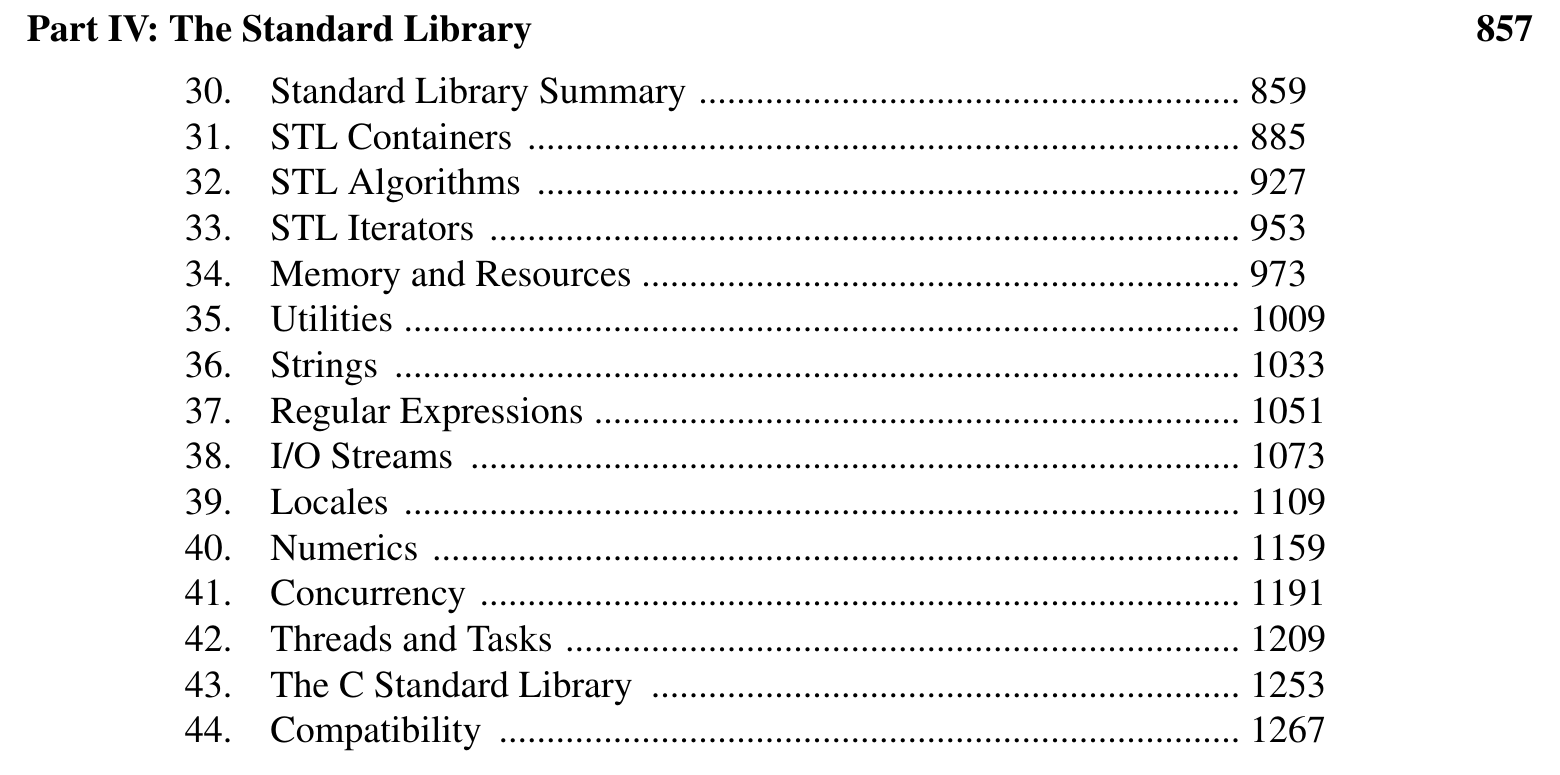
\includegraphics[height=0.7\textheight]{img/summary.png}
\end{frame}

\subsection{Headers}
\begin{frame}
  \frametitle{The header files}
  \centering
  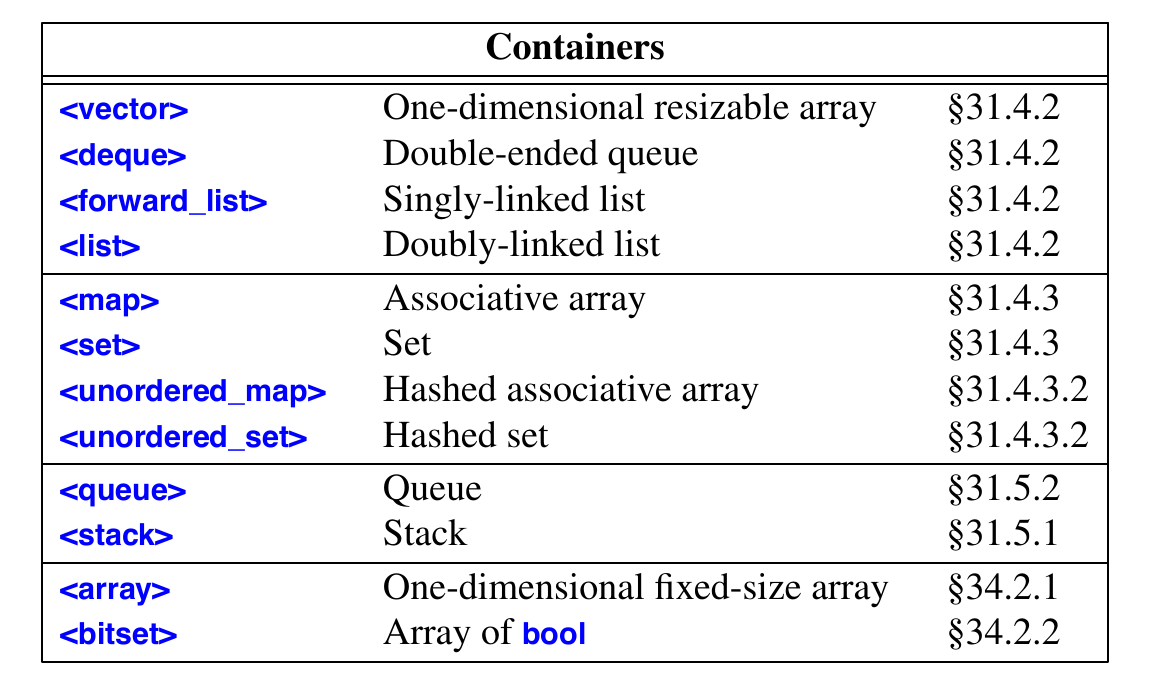
\includegraphics[width=0.7\textwidth]{img/head_01.png}
\end{frame}
\begin{frame}
  \frametitle{The header files}
  \centering
  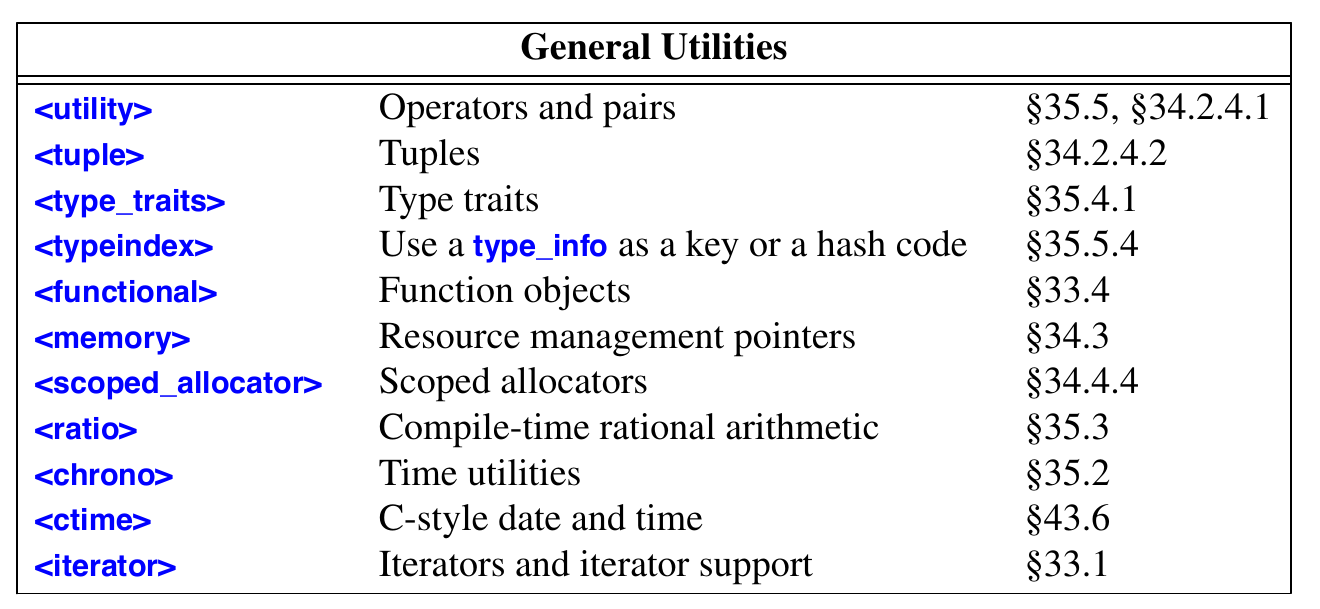
\includegraphics[width=0.7\textwidth]{img/head_02.png}
\end{frame}
\begin{frame}
  \frametitle{The header files}
  \centering
  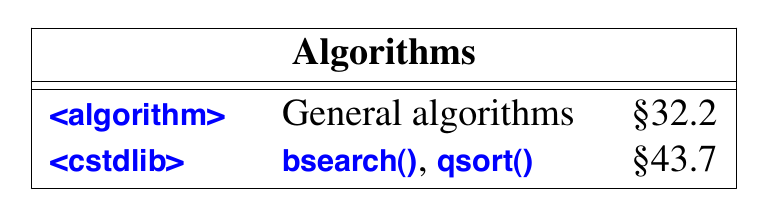
\includegraphics[width=0.7\textwidth]{img/head_03.png}
\end{frame}
\begin{frame}
  \frametitle{The header files}
  \centering
  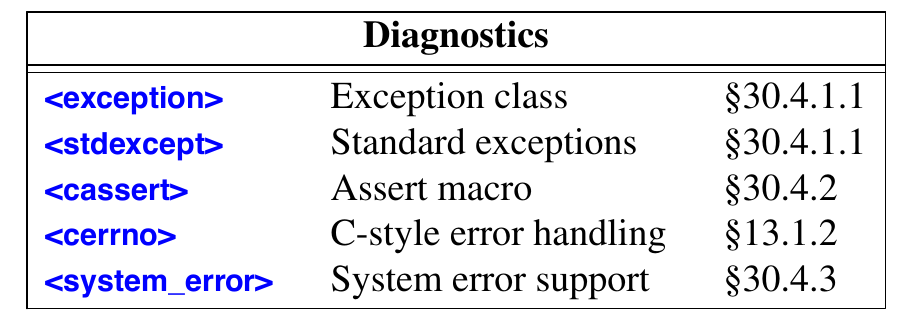
\includegraphics[width=0.7\textwidth]{img/head_04.png}
\end{frame}
\begin{frame}
  \frametitle{The header files}
  \centering
  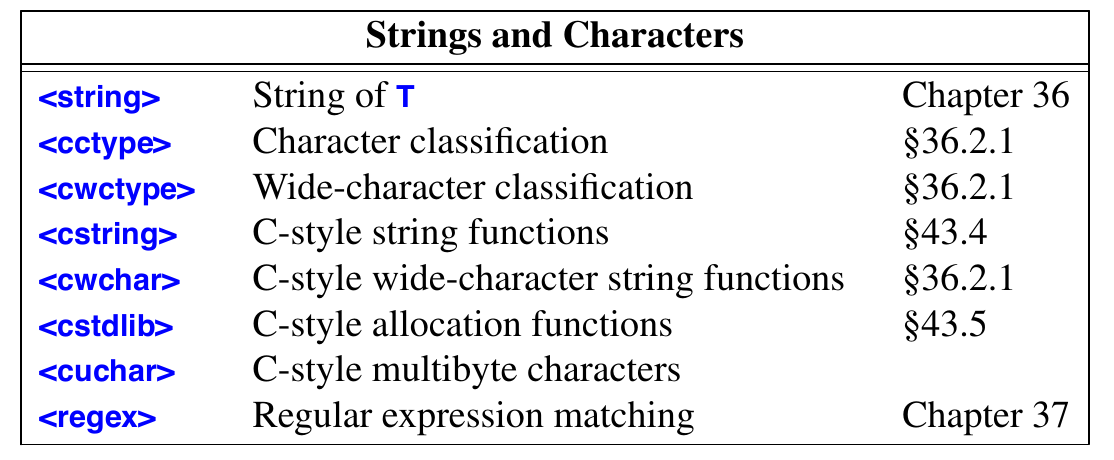
\includegraphics[width=0.7\textwidth]{img/head_05.png}
\end{frame}
\begin{frame}
  \frametitle{The header files}
  \centering
  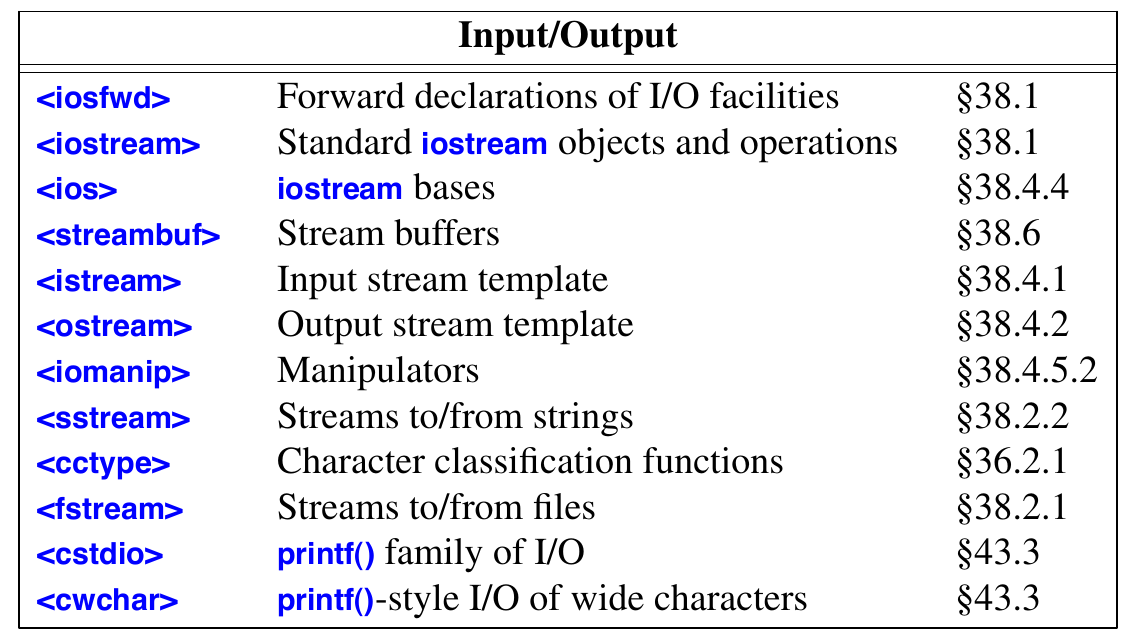
\includegraphics[width=0.7\textwidth]{img/head_06.png}
\end{frame}
\begin{frame}
  \frametitle{The header files}
  \centering
  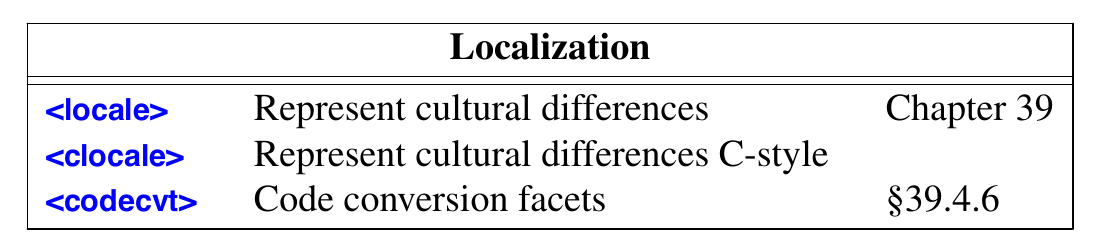
\includegraphics[width=0.7\textwidth]{img/head_07.png}
\end{frame}
\begin{frame}
  \frametitle{The header files}
  \centering
  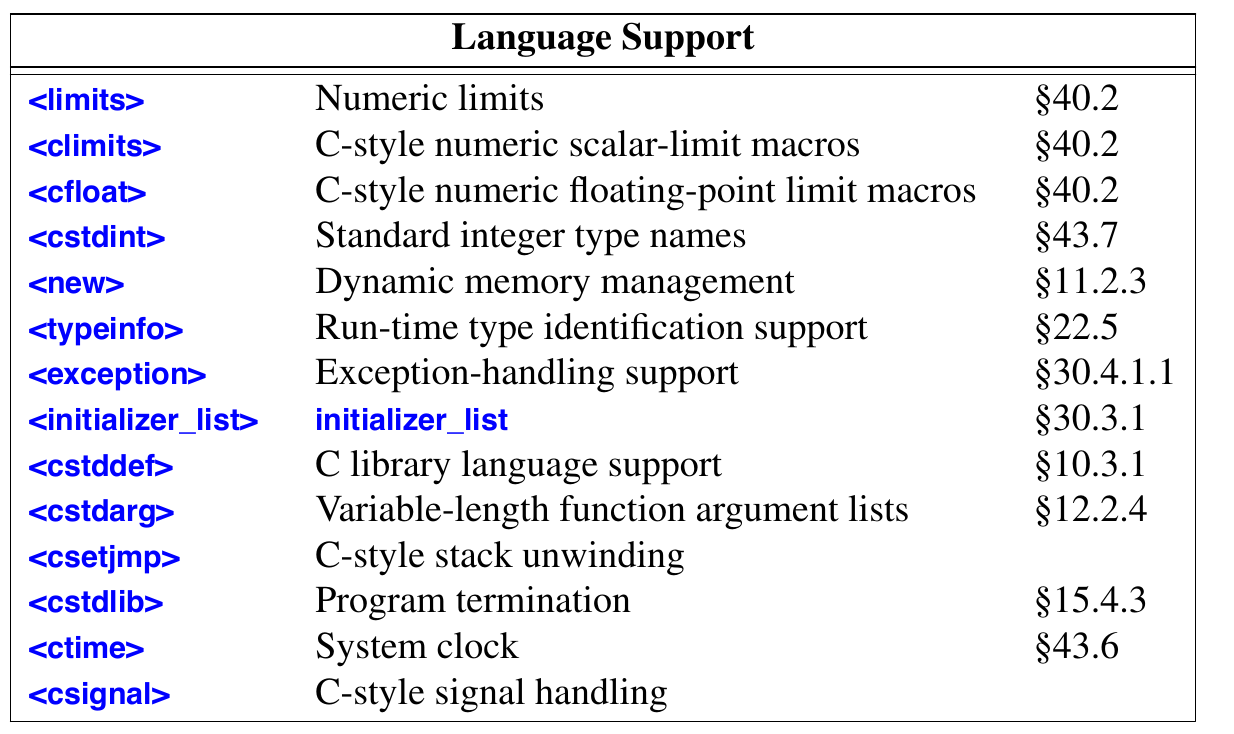
\includegraphics[width=0.7\textwidth]{img/head_08.png}
\end{frame}
\begin{frame}
  \frametitle{The header files}
  \centering
  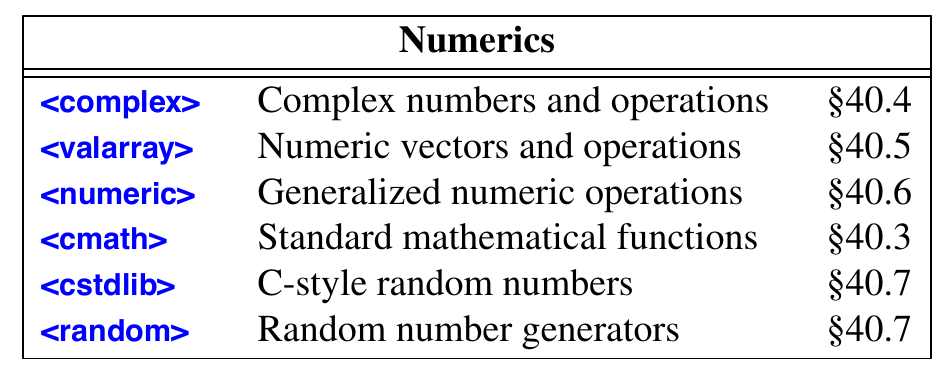
\includegraphics[width=0.7\textwidth]{img/head_09.png}
\end{frame}
\begin{frame}
  \frametitle{The header files}
  \centering
  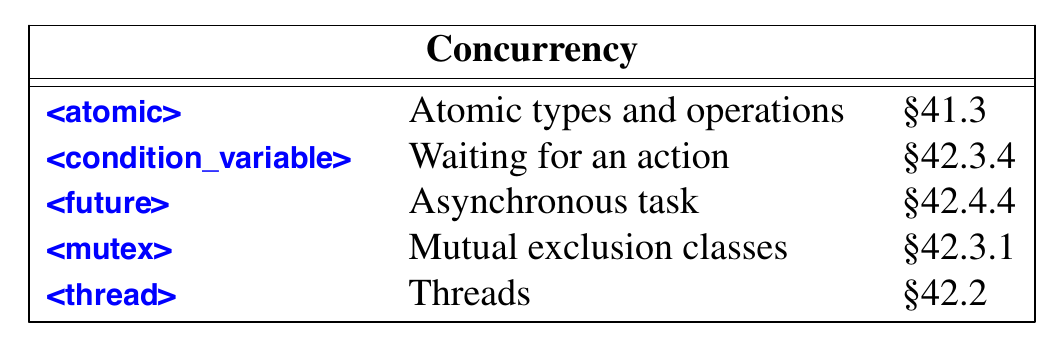
\includegraphics[width=0.7\textwidth]{img/head_10.png}
\end{frame}
\begin{frame}
  \frametitle{The header files}
  \centering
  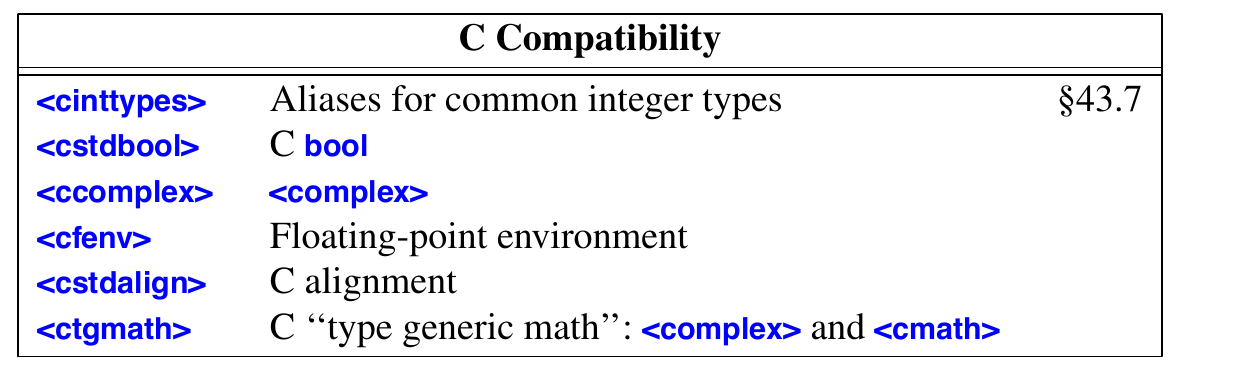
\includegraphics[width=0.7\textwidth]{img/head_11.png}
\end{frame}
\begin{frame}
  \frametitle{The header files}
  \centering
  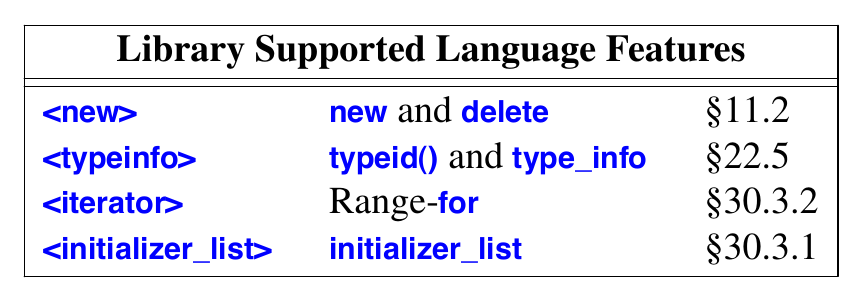
\includegraphics[width=0.7\textwidth]{img/head_12.png}
\end{frame}
\subsection{STL}
\begin{frame}
  \frametitle{We will focus on the STL \smiley}
  \centering
  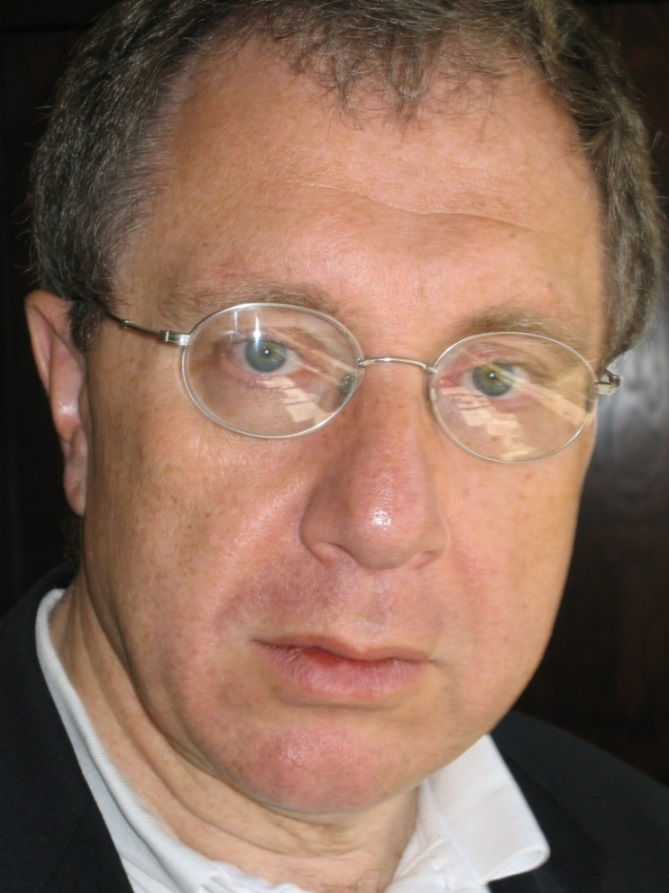
\includegraphics[height=0.7\textheight]{img/alex.jpg}
\end{frame}
\subsection{Concurrency}
\begin{frame}[fragile]
  \frametitle{We will not see the concurrency library \frownie }
\begin{lstlisting}
  int main(){
    // f and g are independent
    f();
    g();
  }
\end{lstlisting}
\end{frame}

\begin{frame}[fragile]
  \frametitle{We will not see the concurrency library  \frownie }
\begin{lstlisting}
  #include <thread>
    
  int main(){
    // f and g are independent
    std::thread t{ f };
    g();
    t.join();
  }
\end{lstlisting}

\end{frame}



\begin{frame}[fragile]
  \frametitle{We will not see the concurrency library \frownie }
\begin{lstlisting}
  #include <future>
    
  int main(){
    // f and g are independent
    auto from_f = std::async( f );
    auto from_g = g();
    ...
    complicated( from_g, from_f.get() );
  }
\end{lstlisting}
\end{frame}

\begin{frame}[fragile]
  \frametitle{We will not see the concurrency library \frownie }
  \framesubtitle{Link  against \texttt{pthread}}
%% \lstset{language=bash}
\begin{lstlisting}
  $ c++ test.cpp -pthread
\end{lstlisting}
\vfill
\begin{lstlisting}
  $ c++ test.cpp -c
  $ c++ test.o -pthread
\end{lstlisting}

\end{frame}

\section{Containers}
\subsection{Introduction}
\begin{frame}
  \frametitle{Containers}
  \begin{block}{Definition}
    A container holds a sequence of objects
  \end{block}
  \vfill
  \begin{block}{Two categories}
    \begin{itemize}
    \item Sequence containers: provide access to sequences of elements
    \item Associative containers: provide associative lookup based on a key
    \end{itemize}
  \end{block}
  \vfill
  \begin{block}{Associative containers}
    \begin{itemize}
    \item Ordered
    \item Unordered
    \end{itemize}
  \end{block}
\end{frame}

\subsection{Sequence containers}
\begin{frame}
  \frametitle{Sequence containers}
  \centering
  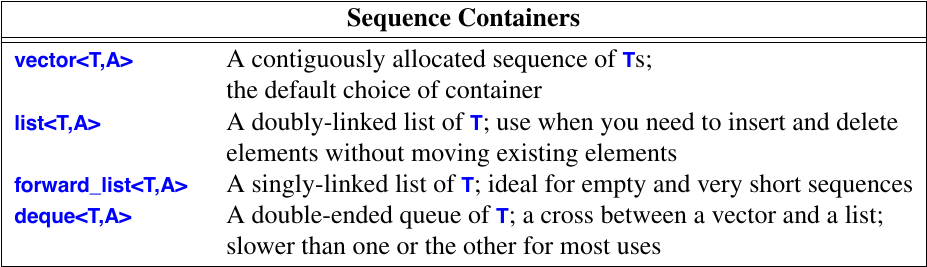
\includegraphics[width=\textwidth]{img/sequence_containers.png}
\end{frame}

\subsection{Associative containers}
\begin{frame}
  \frametitle{Ordered associative containers}
  \centering
  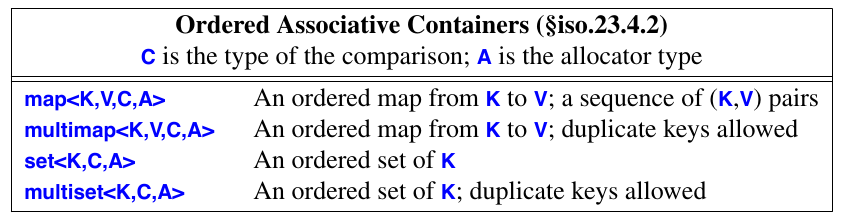
\includegraphics[width=\textwidth]{img/ordered.png}
\end{frame}
\begin{frame}
  \frametitle{Unordered associative containers}
  \centering
  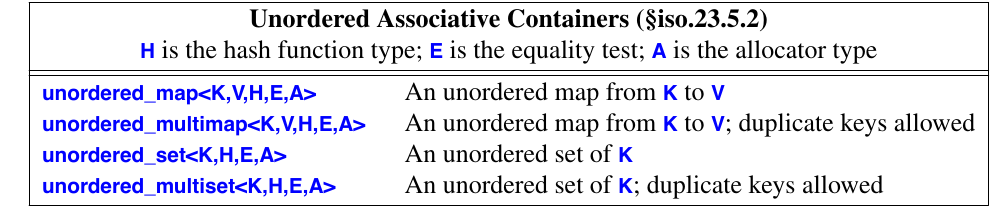
\includegraphics[width=\textwidth]{img/unordered.png}
\end{frame}

\subsection{Container representation}
\begin{frame}
  \frametitle{Array}
  \centering
  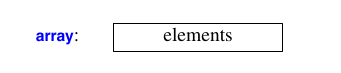
\includegraphics[width=0.5\textwidth]{img/array.png}
\end{frame}

\begin{frame}
  \frametitle{Vector}
  \centering
  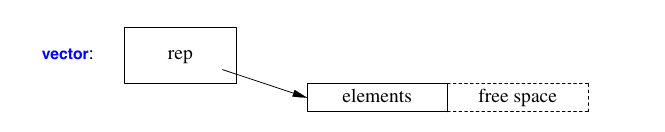
\includegraphics[width=\textwidth]{img/vector.png}
\end{frame}

\begin{frame}
  \frametitle{Forward list}
  \centering
  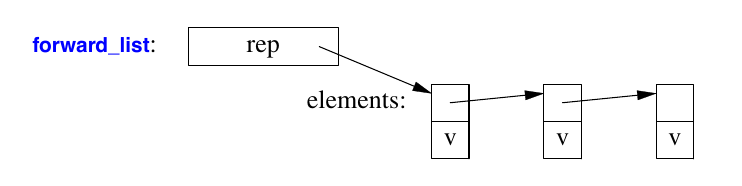
\includegraphics[width=\textwidth]{img/forward_list.png}
\end{frame}

\begin{frame}
  \frametitle{List}
  \centering
  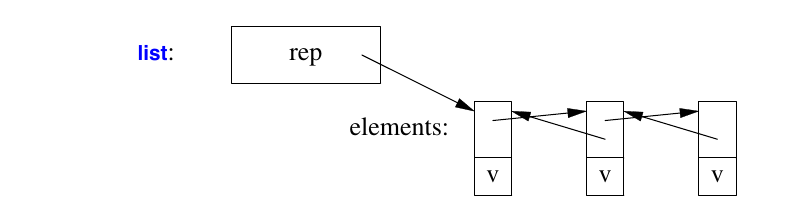
\includegraphics[width=\textwidth]{img/list.png}
\end{frame}

\begin{frame}
  \frametitle{Map}
  \centering
  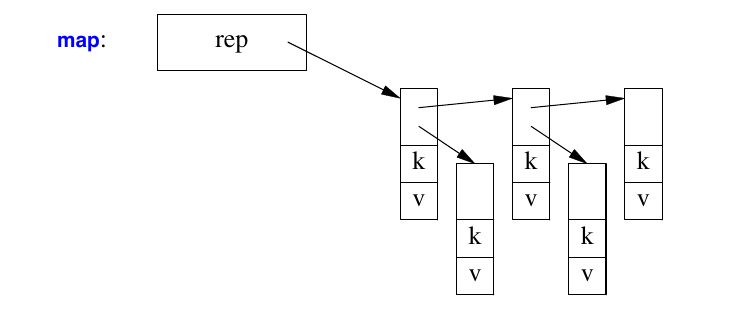
\includegraphics[width=\textwidth]{img/map.png}
\end{frame}

\begin{frame}
  \frametitle{Unordered map}
  \centering
  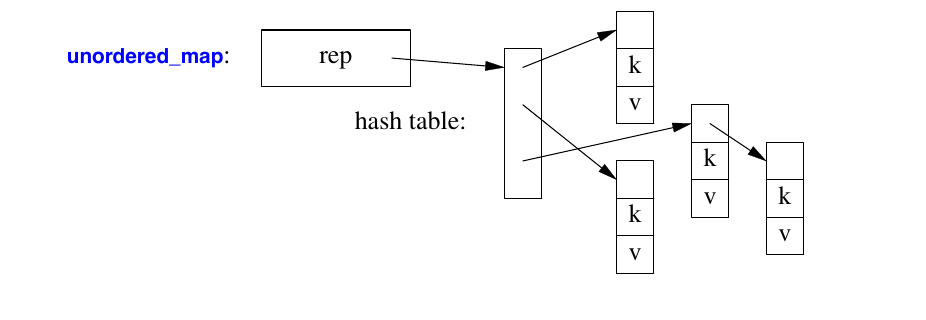
\includegraphics[width=\textwidth]{img/unordered_map.png}
\end{frame}

\subsection{Overview}
\begin{frame}
  \frametitle{Operations and types}
  \centering
  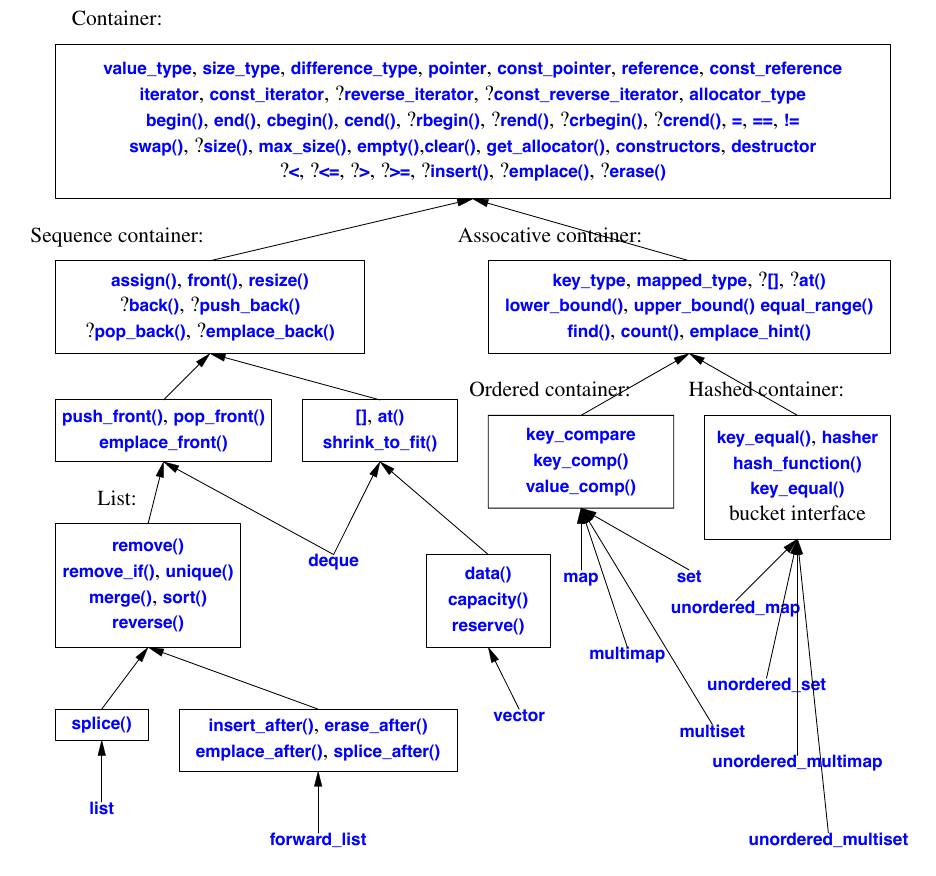
\includegraphics[height=0.95\textheight]{img/members.png}
\end{frame}

\begin{frame}
  \frametitle{Operation complexity}
  \centering
  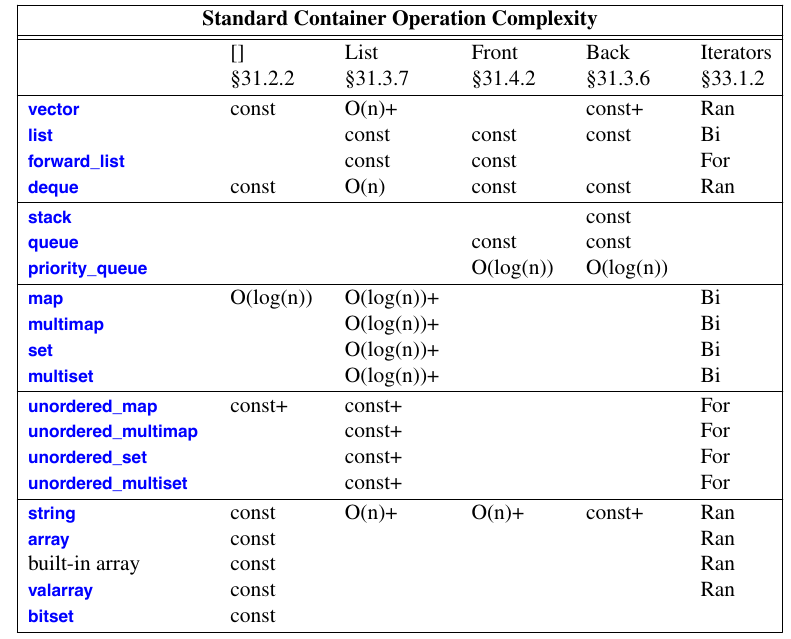
\includegraphics[height=0.9\textheight]{img/complexity.png}
\end{frame}

\subsection{Examples}
\begin{frame}[fragile]
  \frametitle{Prime numbers}
\begin{lstlisting}
#include <vector>

int main(){
  std::vector<int> primes;
  
  primes.emplace_back(2);

  for (int i=3; i<=max; ++i)
    if (is_prime(i))
      primes.emplace_back(i);

  for (const auto& x: primes)
    std::cout << x << std::endl;
}
\end{lstlisting}
\end{frame}

\begin{frame}[fragile]
  \frametitle{Word count}
\begin{lstlisting}
#include <map>
  
int main(){
  std::map<std::string, int> words;
  
  for (std::string s; std::cin>>s;)
    ++words[s];

  for (const auto& x: words)
  std::cout << x.first << ": "
            << x.second << std::endl;
}
\end{lstlisting}
\end{frame}

\begin{frame}[fragile]
  \frametitle{Word count}
\begin{lstlisting}
#include <unordered_map>
  
int main(){
  std::unordered_map<std::string, int> words;
  
  for (std::string s; std::cin>>s;)
    ++words[s];

  for (const auto& x: words)
  std::cout << x.first << ": "
            << x.second << std::endl;
}
\end{lstlisting}
\end{frame}

\section{Iterators}
\subsection{What they are}
\begin{frame}
  \frametitle{What is an Iterator?}
  \begin{block}{Design pattern [GoF]}
    Provide a way to access the elements of an aggregate object sequentially without exposing its underlying representation.
  \end{block}
  \vfill
  \begin{block}{Stepanov}
    Iterator is a coordinate.
  \end{block}
  \vfill
  \begin{block}{A generalization of a pointer}
    \begin{itemize}
    \item indirect access (\texttt{operator*()}, \texttt{operator->()})
    \item operations for moving to point to a new element (\texttt{operator++()}, \texttt{operator--()}) 
    \end{itemize}
  \end{block}
\end{frame}

\subsection{Iterators in the STL}

\begin{frame}
  \frametitle{Iterators in the STL}
  \begin{block}{Their role}
    \begin{itemize}
    \item Iterators are the glue that ties the standard-library alogorithms to their data
    \item Iterators are the mechanism used to minimize an algorithm's dependence on the data structures on which it operates.
      \end{itemize}
  \end{block}
\vfill
  \begin{block}{Alex Stepanov}
    The reason that STL containers and algorithms work so well together is that they know nothing of each other.
    \end{block}
\end{frame}

\begin{frame}[fragile]
  %% \frametitle{How to use iterators}
  \vfill
  \begin{lstlisting}
       while( first != last )
  \end{lstlisting}
  \vfill
\end{frame}


\subsection{Iterator categories}
\begin{frame}
  \frametitle{Iterator categories}
  \centering
  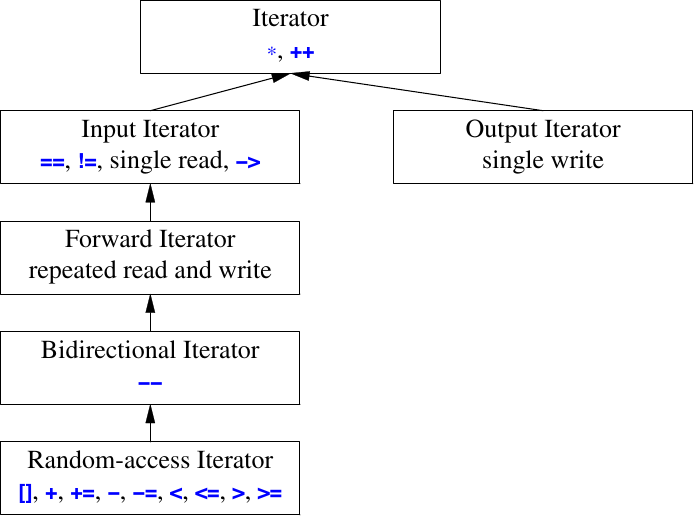
\includegraphics[height=0.8\textheight]{img/iterators.png}
\end{frame}

\begin{frame}[fragile]
  \frametitle{How to implement our own iterator?}
\begin{lstlisting}
  template <typename T>
  class List<T>::Iterator {
    ...
  };
\end{lstlisting}
\end{frame}

\subsection{Our List iterator}
\begin{frame}[fragile]
  \frametitle{How to implement our own iterator?}
\begin{lstlisting}
  #include <iterator>
  ...
  template <typename T>
  class List<T>::Iterator{
    typename List<T>::node* current;
    public:
    using value_type = T;
    using difference_type = std::ptrdiff_t;
    using iterator_category =
      std::forward_iterator_tag;
    using reference = value_type&;
    using pointer = value_type*;
    ...
\end{lstlisting}
\end{frame}

\begin{frame}[fragile]
  \frametitle{How to implement our own iterator?}
\begin{lstlisting}
    ...
    reference operator*() {
      return current->value; }
    pointer operator->() { return &**this; }
    Iterator& operator++() {
      current = current->next;
      return *this;
    }
    friend
    bool operator==(const Iterator&, const Iterator&);
    friend
    bool operator!=(const Iterator&, const Iterator&);
  };
\end{lstlisting}
\end{frame}


\section{Algorithms}
\subsection{Introduction}
\begin{frame}
  \frametitle{STL algorithms}
  \begin{itemize}
  \item about 80 algorithms in \texttt{<algorithm> and <numeric>}
  \item[]
  \item operate on \emph{sequences}
    \begin{itemize}
    \item pair of iterators for inputs $[b:e)$
    \item single iterator for output $[b2: b2+(e-b))$
    \end{itemize}
  \item[]
  \item can take functions or function objects
  \item[]
  \item report failure (e.g. not found) by returning the end of the sequence
  \end{itemize}
\end{frame}
\subsection{Quick examples}
\begin{frame}[fragile]
  \frametitle{Examples}
  \framesubtitle{Sequences}
\begin{lstlisting}
  #include <algorithm>
  #include <vector>
  
  int main(){
    std::vector<double> v1;
    ...
    std::vector<double> v2(v1.size());
    std::sort(v1.begin(), v1.end());
    std::copy(v1.begin(), v1.end(), v2.begin());
  }
\end{lstlisting}
\end{frame}

\begin{frame}[fragile]
  \frametitle{Examples}
  \framesubtitle{Sequences}
\begin{lstlisting}
#include <numeric>
#include <vector>
  
int main(){
  std::vector<double> v1;
  ...
  double sum{0};
  sum = std::accumulate(v1.begin(),v1.end(),sum);
}
\end{lstlisting}
\end{frame}

\begin{frame}[fragile]
  \frametitle{Examples}
  \framesubtitle{User-defined functions}
\begin{lstlisting}
#include <numeric>
#include <vector>

double my_f(const double& a, const double& b){
 if(std::abs(b - 2.2) < 1e-12)
  return a;
 return a+b;
}
int main(){
 std::vector<double> v1;
 ...
 double sum{0};
 sum = std::accumulate(first,last,sum,my_f);
}
\end{lstlisting}

\end{frame}


\begin{frame}[fragile]
  \frametitle{Examples}
  \framesubtitle{Lambda functions}
\begin{lstlisting}
#include <numeric>
#include <vector>
int main(){
 std::vector<double> v1;
 ...
 auto my_f = [](const double& a, const double &b) -> double {
   return ( (std::abs(b-2.2) < 1e-12) ? a : a+b);
 };
 double sum{0};
 sum = std::accumulate(first,last,sum,my_f);
}
\end{lstlisting}
\end{frame}

\begin{frame}[fragile]
  \frametitle{Examples}
  \framesubtitle{Generic lambdas (since C++14)}
\begin{lstlisting}
#include <numeric>
#include <vector>
int main(){
 std::vector<double> v1;
 ...
 auto my_f = [](const auto& a, const auto& b) {
   return ( (std::abs(b-2.2) < 1e-12) ? a : a+b);
 };
 double sum{0};
 sum = std::accumulate(first,last,sum,my_f);
}
\end{lstlisting}

\end{frame}

\begin{frame}[fragile]
  \frametitle{Examples}
  \framesubtitle{Failure check}
\begin{lstlisting}
#include <algorithm>
#include <vector>
  
int main(){
  std::vector<double> v1;
  ...
  auto it = std::find(v1.begin(), v1.end(), 2.2);

  if(it != v1.end())
    std::cout << "found " << *it << std::endl;
  else
    std::cout << "not found\n";
}
  
\end{lstlisting}
\end{frame}

\section{Function objects}
\subsection{Introduction}
\begin{frame}
  \frametitle{Function objects}
  \begin{itemize}
  \item defined in \texttt{<functional>}
  \item[]
  \item comparison criteria
  \item[]
  \item predicates (functions returning \texttt{bool})
  \item[]
  \item arithmetic operations
  \end{itemize}
\end{frame}
\begin{frame}
  \frametitle{Predicates}
  \centering
  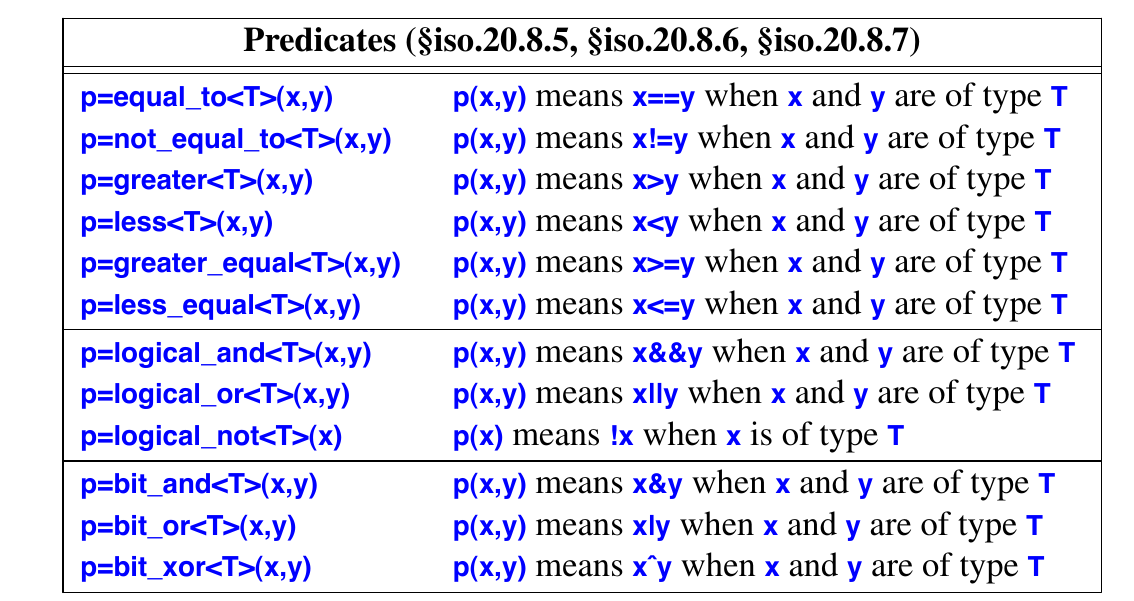
\includegraphics[width=0.8\textwidth]{img/predicates.png}
\end{frame}
\begin{frame}
  \frametitle{Arithmetic operations}
  \centering
  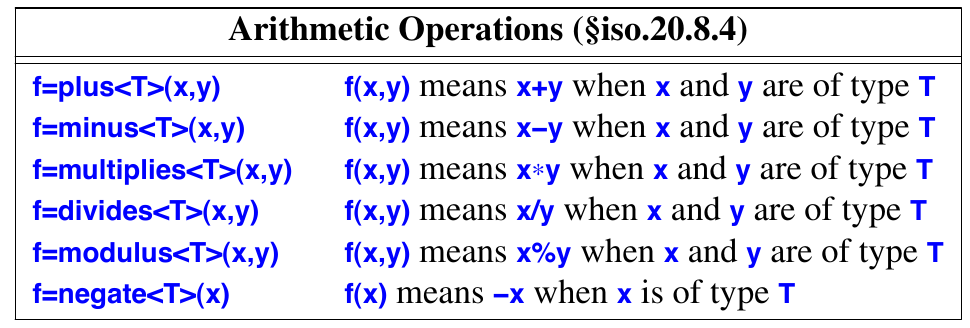
\includegraphics[width=0.8\textwidth]{img/arithmetic.png}
\end{frame}

\subsection{Examples}
\begin{frame}[fragile]
  \frametitle{Decreasing sort}
\begin{lstlisting}
#include <algorithm>
#include <vector>
#include <functional>
  
int main(){
  std::vector<double> v1;
  ...
  std::sort(v1.begin(), v1.end(),
            std::greater<double>{});
}
\end{lstlisting}
\end{frame}

\begin{frame}[fragile]
  \frametitle{My comparison}
\begin{lstlisting}
#include <algorithm>
#include <vector>
  
template <typename num>
struct my_comparison{
  bool operator()(const num& a, const num& b) { return a > b;}
};
  
int main(){
  std::vector<double> v1;
  ...
  std::sort(v1.begin(), v1.end(),
            my_comparison<double>{});
}
\end{lstlisting}
\end{frame}

\begin{frame}[fragile]
  \frametitle{Lambda}
\begin{lstlisting}
#include <algorithm>
#include <vector>

int main(){
  std::vector<double> v1;
  ...
  std::sort(v1.begin(), v1.end(),
           [](const auto& a, const auto& b)
              { return a>b; } );
}
\end{lstlisting}
\end{frame}

\section*{}
\begin{frame}
  \centering
  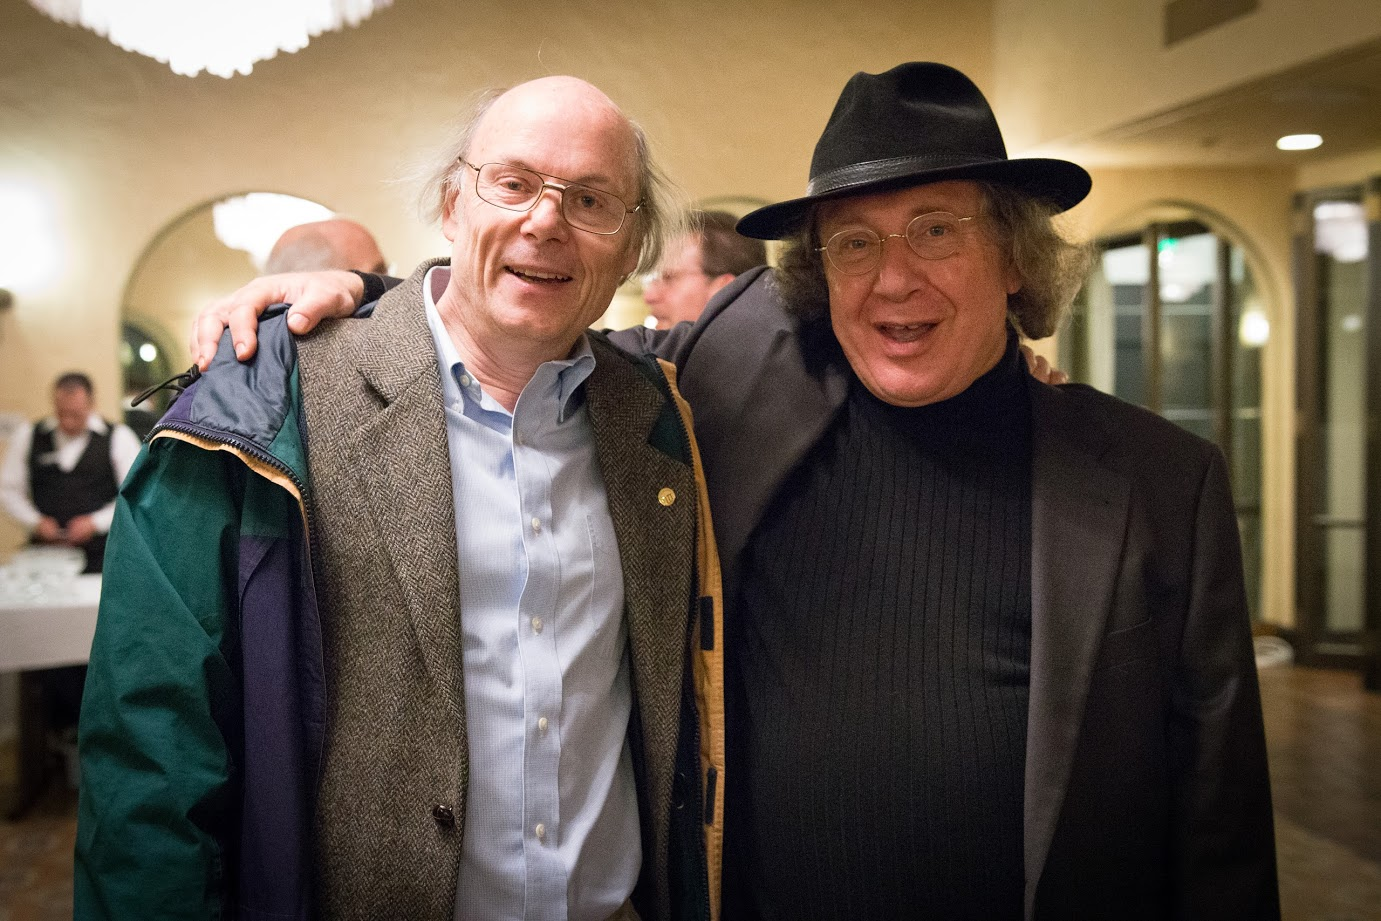
\includegraphics[width=0.8\textwidth]{img/alexfest.jpg}
\end{frame}
			
\defbeamertemplate*{footline}{for appendix}
{
  \leavevmode%
  \hbox{%
  \begin{beamercolorbox}[wd=.333333\paperwidth,ht=2.25ex,dp=1ex,center]{author in head/foot}%
    %\usebeamerfont{author in head/foot}\insertshortauthor
    \usebeamerfont{author in head/foot}\insertshortauthor~~\insertshortinstitute
  \end{beamercolorbox}%
  \begin{beamercolorbox}[wd=.333333\paperwidth,ht=2.25ex,dp=1ex,center]{title in head/foot}%
    \usebeamerfont{title in head/foot}\insertshorttitle
  \end{beamercolorbox}%
  \begin{beamercolorbox}[wd=.333333\paperwidth,ht=2.25ex,dp=1ex,right]{date in head/foot}%
    \usebeamerfont{date in head/foot}\insertshortdate{}\hspace*{2em}
%    \insertframenumber{} / \inserttotalframenumber\hspace*{2ex} 
  \end{beamercolorbox}}%
  \vskip0pt%
}
\usebackgroundtemplate{}
%% \input{tex_files/bckup_slides.tex}
				
\end{document}
